\documentclass[11pt]{article}

\usepackage{amsmath}
\usepackage{amssymb}
\usepackage{array}
\usepackage{caption}
\usepackage{graphicx}

\usepackage[autostyle, english=american]{csquotes}
\MakeOuterQuote{"}
\captionsetup[table]{skip=1pt}

\newcolumntype{M}[1]{>{\centering\arraybackslash}m{#1}}

% margins
\topmargin=-0.45in
\evensidemargin=0in
\oddsidemargin=0in
\textwidth=6.5in
\textheight=9.0in
\headsep=0.25in

\title{605.744: Information Retrieval \\ Problem Set (Module 8)}
\author{Sabbir Ahmed}
\date{\today}

\begin{document}
\maketitle

    \begin{enumerate}

        \item (30\%) Give a short definition or explanation of the following concepts:
        \begin{itemize}
            \item web spam
            \item Broder's taxonomy
            \item out-degree
            \item robots exclusion protocol
            \item priority queue (in the context of web crawling)
        \end{itemize}

        \textbf{Answer:}

        \item (20\%) Describe in your own words the process described in the course text to efficiently identify near duplicate documents in a large collection.

        \textbf{Answer:}

        \item For this problem work with the directed web graph shown below. In the graph there are six nodes: Y, B, F, G, T, R (for the websites Yahoo, Bing, Facebook, Google, Twitter, and Reddit). Use a teleport probability of 0.20. Assume no other pages or links exist beside those shown in the figure.

        % \begin{figure}[!ht]
        %     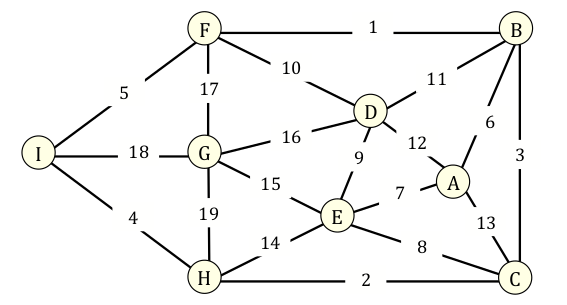
\includegraphics[scale=0.35]{statics/graph.png}
        %     \centering
        % \end{figure}

        \begin{enumerate}
            \item (15\%) Provide (i.e., write) the six recurrence equations that indicate how to iteratively calculate the PageRank score of each page at time t given scores from time t-1.
            
            \textbf{Answer:}

            \item (25\%) Using the brute-force iterative method of calculation shown in the video lecture calculate two iterations of PageRank scores for each page in the graph. Be sure to show scores at times t=0, t=1, and finally at t=2. Report scores using three digits of precision (e.g., 0.247, not 0.2 or 0.24696485932). Show work and do not merely provide a table of values.
            
            \textbf{Answer:}

            \item (5\%) Which page (or pages) has/have the lowest PageRank score after two iterations?
            
            \textbf{Answer:}

            \item (5\%) Which page (or pages) has/have the highest PageRank score after two iterations?
            
            \textbf{Answer:}

        \end{enumerate}

    \end{enumerate}

\end{document}
